\chapter{Étude préalable} \label{Chapter2}

\section{Méthode d’analyse et de conception : Merise}
Une méthode est la mise en œuvre de plusieurs étapes (méthodologiques), d'une démarche, de principes, d'outils.

La méthode MERISE est pour cela une méthodologie qui propose des étapes pour la mise en place et la conduite de projets informatiques. Le terme MERISE, acronyme signifiant méthode d'études et de réalisations de systèmes informatiques pour les entreprises, est le plus couramment et le plus largement utilisé pour la conception et la réalisation de bases de données en France.
Cette méthode vise à remplacer le système de gestion manuelle d'une organisation par un système automatisé de traitement de l'information. Elle vise, d'une part, à démontrer les problèmes potentiels du système existant et, d'autre part, à apporter des améliorations à ce dernier. Les facteurs considérés dans l'étude sont la collecte, le stockage, le traitement et la transmission de l'information.

\begin{figure}[ht!]
    \centering
    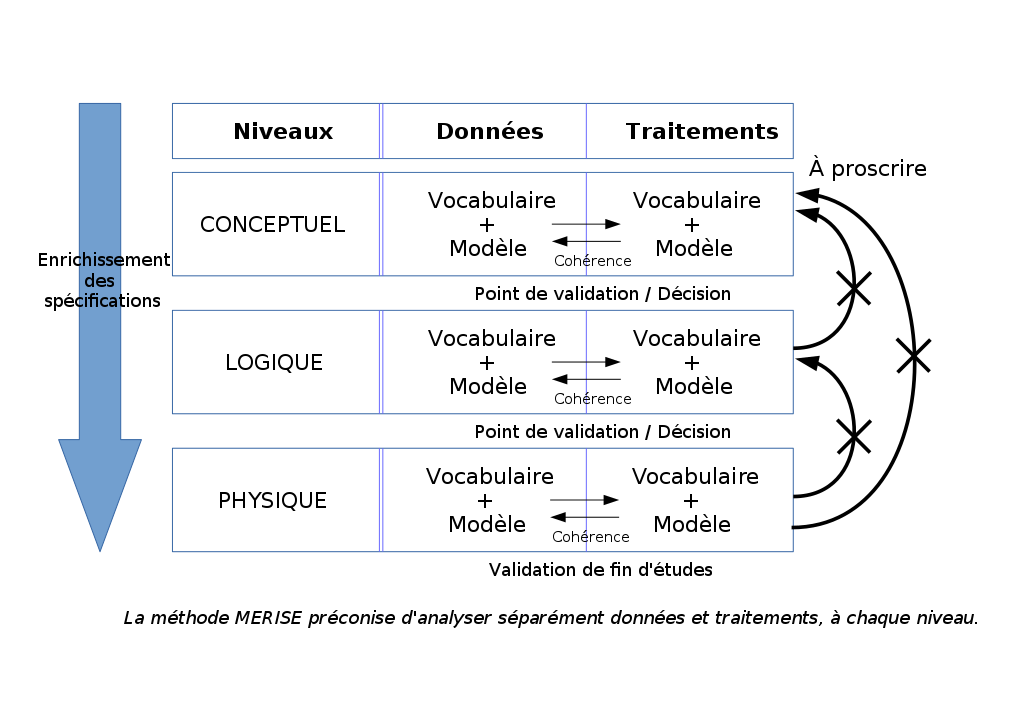
\includegraphics[keepaspectratio=true,scale=0.3]{Figures/merise.png}
    \caption{Méthode MERISE}
    \label{fig:merise}
\end{figure}

Ainsi, MERISE permet d'entreprendre une étude de l'existant et de passer à la conception proprement dite, si cette dernière est la solution, en procédant par exemple comme suit :

\paragraph{Étude de l'existant :} Ici on décrit de manière détaillée la structure existante qui décrit la situation réelle de l'organisation et son fonctionnement.
\paragraph{Analyse et évaluation de l'existant :} Identification des problèmes et des moyens de les résoudre.
\paragraph{Conception et mise en place du nouveau système :} proposer un modèle qui aboutit à la base de données ou encore proposer des interfaces et des programmes en utilisant certains langages de programmation et systèmes de gestion de bases de données.


Toutes ces étapes peuvent être résumées dans la figure \ref{fig:merise}.


\section{Analyse du problème}
\subsection{Contexte}
Le but est d'améliorer la gestion des stocks d’une maison. On va créer une application pour gérer efficacement leurs inventaires. Cette application permettra de gérer à la fois les articles achetés, et les produits, mais aussi de gérer l'inventaire hebdomadaire des lots par les dirigeants. Nous avons donc créé le cahier des charges suivant, qui décrit notre démarche.

\subsection{Analyse et aboutissements}
Pour des raisons de simplicité, on considère que les \textbf{produits} que nous stockerons dans la base de données sont tous des produits destinés uniquement à être consommés (viande, fruit, etc..).

Chaque produit a un identifiant, un libellé et une brève description, et chacun d'eux appartient à une \textbf{catégorie} spécifique. Il est possible de définir des caractéristiques communes entre certains produits. Ces caractéristiques communes peuvent être divisées en deux groupes : le premier est lié à la \textbf{forme} du produit (poids, hauteur, volume), et le second contient des \textbf{informations} générales telles que la date d'expiration, le prix unitaire, la quantité, et la température (minimale et maximale). Cet inventaire est créé indépendamment pour chaque utilisateur afin que les données de chacun soient séparées de celles des autres.

Chaque produit doit être inscrit à l'inventaire de la maison (\textbf{stock}). Il a un identifiant, un nom et la quantité de produit disponible. Il est acheté auprès d'une ou plusieurs entreprises à la fois. Ici, nous considérons que l'\textbf{entreprise} ne vend qu'un seul type de produits. Une entreprise peut être présente dans plus d'une \textbf{ville}. Ainsi, une ville peut contenir plusieurs entreprises.

Quand un \textbf{utilisateur} achète un nouveau produit ou augmente la quantité d'un produit. Nous le mettons dans le stock. Chaque produit comporte la date à laquelle il a été ajouté, ainsi qu'une date à laquelle nous le récupérons, au cas où il serait périmé ou que nous ne l'aurions plus en stock.

Chaque fois qu'un produit est ajouté au stock, l'utilisateur peut effectuer un \textbf{contrôle} pour vérifier si le produit est périmé ou non. L'utilisateur peut également vérifier, de temps en temps, la disponibilité d'un certain produit.

Chaque processus de contrôle doit être suivi d'une brève description de ses résultats. Bien évidemment, les résultats de ces contrôles peuvent être variés. Mais, pour simplifier, nous ne considérons dans ce projet que ces résultats typiques : produit périmé, produit non disponible en stock, produit disponible en stock.

\subsection{Fonctionnalités}

\paragraph{Parcourir les articles :} L'utilisateur parcourt les articles disponibles dans son inventaire.
\paragraph{Insérer un élément :} L'utilisateur insère un élément dans son inventaire.
\paragraph{Supprimer un élément :} L'utilisateur supprime un élément de l'inventaire.
\paragraph{Modifier l'élément :} L'utilisateur peut modifier les propriétés d'un élément.
\paragraph{Login :} Se connecter au système.
\paragraph{Logout :} Se déconnecter du système
\paragraph{Modifier l'identifiant et le mot de passe :} L'utilisateur peut changer son identifiant et son mot de passe.

\section{L’identification des besoins}
\subsection{Les besoins fonctionnels}
Le système doit assurer les fonctionnalités suivantes :

\paragraph{1. Le système doit permettre aux utilisateurs de modifier leurs mots de passe par mesure de sécurité.}
\paragraph{2. Le système doit permettre aux utilisateurs d'enregistrer toutes les informations relatives aux produits achetés, à ceux qui restent dans le stock.}
\paragraph{3. Le système doit être capable d'exporter tous les enregistrements stockés afin de les analyser.}

\subsection{Les besoins non fonctionnels}
\paragraph{Ergonomie et Convivialité}
L’application devra offrir aux utilisateurs un cadre de travail organiser et harmonieux. Par des interfaces graphiques claires et lisibles, la possibilité d’effectuer des recherches facilement, et de sauvegarder leurs données.

\paragraph{Facilité d’utilisation et facteur humain}
Nous voulons faciliter l’utilisation de l’application en simplifiant d’abord sa manipulation, ensuite en proposant un guide d’utilisation précis, afin qu’il soit utilisable par n’importe quel agriculteur. Aucune compétence en informatique ne sera nécessaire pour manipuler ce produit. L’utilisateur aura un accès à un menu "aide" où il pourra s’informer sur l’application, et communiquer ses difficultés ou préoccupations rencontrées.

\paragraph{Sécurité}
Chaque utilisateur aura un compte privé et un mot de passe qu’il devra fournir pour accéder au site, et ce mot de passe pourra au besoin être modifier pour assurer plus de sécurité.

\paragraph{Le système ne doit pas occuper plus que l'espace requis pour un programme normal à l'espace disque.}


\section{L’analyse des besoins : Identification des acteurs}
L'application sera généralement utilisée par deux types d'utilisateurs, un utilisateur à domicile et un administrateur système. Les utilisateurs à domicile sont des personnes qui utilisent le système pour leur inventaire quotidien. Les administrateurs du système constituent un groupe très restreint d'utilisateurs qui ont accès à l'ensemble du système et peuvent en modifier tous ses aspects.

% \section{Conclusion}
